\documentclass[]{article}

\usepackage{titlesec}
\usepackage[cache=false]{minted}
\usepackage{listings}
\usepackage{graphicx}
\usepackage{float}
\usepackage{amsmath}
\usepackage[autostyle]{csquotes}
\usepackage{graphicx}  
\usepackage{acronym}
% \usepackage{svg}

% \titleformat{\section}[display]
% {\normalfont\bfseries}{}{0pt}{\Large}

% \titleformat{\subsection}[display]
% {\normalfont\bfseries}{}{0pt}{\Large}

\newcommand{\norm}[1]{\lvert \lvert #1 \rvert \rvert}

%opening
\title{Automatic Measurement of Cartilage Thickness in the Human Knee}
\author{Simon Westfechtel, B.Sc.}

\begin{document}
	
	\maketitle
	
	\section{Introduction}
\label{sec:Introduction}
This paper seeks to discuss different methods to automate the measurement of cartilage thickness in the human knee using MRI scans. The methods are based on previous work by Wolfgang Wirth and Felix Eckstein. \cite{wirth2008technique}
\par\noindent
All computational methods make use of segmented MRI scans of the human knee, from the OAI dataset, and are written in Python. More precisely, there were two distinct sets of segmentations used: One set of manually segmented images, containing 507 samples, and one set of automatically segmented images, containing 24,783 samples. The set of automatic segmentations contained samples from the entire OAI dataset, i.e. over all time periods. Manual segmentations are stored as MHD and automatic segmentations as NIFTI files, respectively, which can be read and converted into Numpy arrays using the SimpleITK library. These arrays map each point in the three-dimensional space of the scan to an integer encoding, meaning for example points belonging to the femoral cartilage are assigned a value of 3. This makes isolating and extracting the cartilage volumes straightforward. Four different methods have been developed to determine mean cartilage thickness, plus other statistical measures. Thickness was measured for different subregions of the cartilage plate, which were determined as referenced in \cite{wirth2008technique}. For a more detailed description of the procedure, refer to appendix \ref{sec:Subregions}. 

\section{Mean cartilage thickness using meshes}
\label{sec:Meshes}
This is a three-dimensional approach using meshes and normal vectors to determine the mean thickness of a cartilage volume. The main idea is building an upper and a lower mesh, and calculating the average distance between the two, for example by ray tracing along the normal vectors of the lower mesh against the upper mesh. Other methods, like a K-D-tree nearest neighbour search, are also possible. This works well for the tibial cartilage, because due to its physical shape, it is possible to simply group each point by $x$ and $y$ coordinates and add the point with the highest (lowest) $z$ coordinate to the upper (lower) mesh. The result is two point clouds consisting of vectors $(x, y, z)$, as seen in figure \ref{fig:tibial_point_cloud} (red points make up the upper cloud, green the lower). These can then be converted into polygon meshes using the delaunay algorithm, which in turn allows for determining the normal vectors of the respective meshes. Mean cartilage thickness can be calculated by tracing along the normal vectors of the lower mesh against the upper mesh. For other methods not making use of the normals, like the previously mentioned nearest neighbour search, the delaunay conversion is optional. 
\begin{figure}[htb!]
	\centering
	\includegraphics[width=\linewidth]{./figures/s2}
	\caption{Point clouds of the tibial cartilage}
	\label{fig:tibial_point_cloud}
\end{figure}
\par
The femoral cartilage makes things a bit more tricky. Due to its shape, building an upper and lower mesh is not trivial, because while for the tibial cartilage, there was only one respective vector for each coordinate pair $(x, y)$, there may now be multiple for the areas where the volume describes a curve, so just taking the minimum or maximum $z$ coordinate no longer suffices. Using the previous approach results in point clouds where some areas are left bare, as illustrated in figure \ref{fig:femoral_point_cloud}. One solution, used in this approach, is splitting the volume into parts, and rotating the curved sections, such that it is once again possible to choose points according to the $z$ coordinate. For a detailed description of how this splitting is achieved, refer to appendix \ref{sec:Splitting}. This allows for building an upper and lower point cloud and corresponding delaunay mesh for each part, calculating the mean distance in the same manner as before (aka ray tracing), and finally combining the results.
\begin{figure}[htb!]
	\centering
	\includegraphics[width=\linewidth]{./figures/s4}
	\caption{Point clouds of the femoral cartilage}
	\label{fig:femoral_point_cloud}
\end{figure}

\section{Mean cartilage thickness using ray tracing from a central point}
\label{sec:Raytracing}
This is a three-dimensional approach using ray tracing along normal vectors to determine the mean thickness of a cartilage volume. This is another proposed solution to the previously discussed issue with the shape of the femoral cartilage volume. Instead of using meshes, this approach takes a central point underneath or above the cartilage and utilizes ray tracing from that point against the volume to discover intersection points. The central point is determined by calculating the halfway points between minimum and maximum $x$, $y$ and $z$ coordinates of the cartilage volume, respectively.
\par
A sphere is constructed around the central point, and each of its normal vectors gets extended until it hits the cartilage point cloud, or a maximum number of iterations is reached. If a point is hit, it is saved and the vector again gets extended until it doesn't hit any points anymore, i.e. it is extended past beyond the cartilage. The distance between the first and last point hit is calculated and added to the result set. This way, it is possible to determine the average thickness of the cartilage. One issue with this approach is that it is computationally expensive, as intersection problems tend to be; in essence, there is a trade-off between accuracy and runtime: The more vectors are used for the ray tracing, the more accurate the result is going to be, but each added vector makes the computation more expensive. The resolution of the sphere was set to 30 $\times$ 30, resulting in $30 + 29 \cdot 28 = 842$ normal vectors. No optimization analysis has been performed as of yet.
\begin{figure}[htb!]
	\centering
	\includegraphics[width=\linewidth]{./figures/s5}
	\caption{Ray tracing against the femoral cartilage using a central sphere}
	\label{fig:femoral_sphere}
\end{figure}

\section{Mean cartilage thickness using two-dimensional function fitting}
\label{sec:Function_fitting}
\subsection{Determine thickness via function normals}
\label{sec:Normals}
This is a two-dimensional approach using a least-squares fit of single cartilage layers to determine the mean thickness of a cartilage volume. As the MRI scans consist of a number of slice exposures, it is possible to do the thickness calculation layer by layer. For each layer, a polynomial function gets fitted over the data points, i.e. through the middle of the volume, and a variable number of normals is calculated along the fitted function. For each normal, the inner- and outermost intersection points with the cartilage are determined, and the distance between these to points is added to the result set, as illustrated in figure \ref{fig:normals}.
\begin{figure}[htb!]
	\centering
	\includegraphics[width=\linewidth]{./figures/normals}
	\caption{Normals along a two-dimensional least squares fit}
	\label{fig:normals}
\end{figure} 

\subsection{Determine thickness via integration/function values}
\label{sec:Integration}
This is another two-dimensional variant, where two functions are fitted over the data points, i.e. not through the middle of the volume but rather along the outlines of the volume, as illustrated in figure \ref{fig:integration}. The distance between the functions, i.e. the thickness of the cartilage, can then easily be calculated, for example by integrating both functions and taking the difference ($\int f(x) dx - \int g(x) dx$), or calculating the difference between the function values for every $x$ value ($[\sum_{x_i = 0}^{max(x)} f(x_i) - g(x_i)] \cdot \frac{1}{max(x)}$).
\par
One issue with both of these approaches is that the function fitting may not work well for certain shapes, especially for layers where the number of data points is very sparse.
The degree for the polynomial fit was chosen as four. This is because in practice, no layer is going to have more than two inflection points (layers of the femoral cartilage can generally be approximated by a second-order polynom, while the layers of the tibial cartilage volume follow a third-order form.) and choosing a higher degree than needed is undesirable (overfitting, Runge's phenomenom, etc). While in theory, a degree of two and three, respectively, would be sufficient, it has been set to four to accomodate for edge cases where a lower-order fit might yield poor or no results, e.g. for the layers on the edges of the volume, and the higher flexibility that comes with a higher degree is beneficial.
\begin{figure}[htb!]
	\centering
	\includegraphics[width=\linewidth]{./figures/integration}
	\caption{Two functions fit over the outlines of a tibial cartilage slice exposure}
	\label{fig:integration}
\end{figure}
	\appendix
	\section{Determination of the cartilage subregions}
\label{sec:Subregions}
As proposed by Wirth \& Eckstein, the central weight-bearing zones of the medial / lateral femoral cartilage are divided into three subregions each (central, internal and external), while the two cartilage plates of the medial / lateral tibia are divided into five subregions each (central, internal, external, anterior, posterior). For nomenclature, refer to the table of acronyms below. 
\subsection{Determination of the femoral subregions}
Let the central weight-bearing zones be represented by two point clouds $LF'$ and $MF'$. For both central weight-bearing zones, each subregion should encompass approximately 33\% of the surface. This was achieved in practice by splitting the zones into three parts along the y-axis; two splitting points $p_1, p_2$ are chosen arbitrarily, such that $\min_{y} LF'/MF' < p_1 < p_2 < max_{y} LF'/MF', p_1 = \frac{\max_{y} LF'/MF' - \min_{y} LF'/MF'}{3}, p_2 = 2 \cdot p_1$. $p_1$ and $p_2$ are then iteratively moved along the y-axis until the constraint is satisfied, i.e. 33\% of all data points lie left of $p_1$, 33\% lie between $p_1$ and $p_2$ and 33\% lie right of $p_2$.
\begin{algorithm}
	\caption{Determination of central weight-bearing subregions}
	\label{algo:cwbzRegions}
	\begin{algorithmic}[1]
		\Procedure{CWBZRegions}{P}
		\State $P \gets \text{point cloud}$
		\State $p_1 \gets (\max_{y} P - \min_{y} P) / 3$
		\State $p_2 \gets p_1 \cdot 2$
		\State $P_1 \gets \{\:(x,y,z) \in P' \subset P \:|\: y < p_1\:\}$
		\State $P_2 \gets \{\:(x,y,z) \in P' \subset P \:|\: p_1 < y < p_2\:\}$
		\State $P_3 \gets \{\:(x,y,z) \in P' \subset P \:|\: p_2 < y\:\}$
		\Repeat
			\If{$\lvert P_1 \rvert \div \lvert P \rvert > .33$}
				\State $p_1 \gets p_1 - 1$
			\Else
				\State $p_1 \gets p_1 + 1$
			\EndIf
			\If{$\lvert P_2 \rvert \div \lvert P \rvert > .33$}
				\State $p_2 \gets p_2 - 1$
			\Else
				\State $p_2 \gets p_2 + 1$
			\EndIf
			\State $P_1 \gets \{\:(x,y,z) \in P' \subset P \:|\: y < p_1\:\}$
			\State $P_2 \gets \{\:(x,y,z) \in P' \subset P \:|\: p_1 < y < p_2\:\}$
			\State $P_3 \gets \{\:(x,y,z) \in P' \subset P \:|\: p_2 < y\:\}$
		\Until{$\lvert P_1 \rvert \approx \lvert P_2 \rvert \approx \lvert P_3 \rvert$}
		\State
		\Return $p_1, p_2$
		\EndProcedure
	\end{algorithmic}
\end{algorithm}
\subsection{Determination of the tibial subregions}
As proposed by \cite{wirth2008technique}, each plate of the tibial cartilage can be divided into five subregions (central, internal, external, anterior and posterior).
For each plate, an ellipse around the centre of the plate encompassing approximately 20\% of the plate's surface, represents the central subregion, and four triangles of variable size surrounding the ellipse represent the internal, external, anterior and posterior subregions. Let the lateral / medial tibial cartilage plates be represented by two point clouds $LT$ and $MT$. For each point cloud, the centre of gravity $c$ is determined through simple K-Means-Clustering with a single cluster, i.e. the mean of all data points of the point cloud. Two ellipses around the centres of gravity are defined as $E_L = (c_T, r_T)$ and $E_M = (c_M, r_M)$, where $c_x$ is the centre and $r_x$ is the radius of the ellipse. The ellipse therefore defines a subset of the respective cartilage plate, such that $E_x \subset xT, E_x := \{\:(x,y,z) \in E_x \:|\: \norm{(x,y,z) - c_x} \leq r_x\:\}, \lvert E_x \rvert \div \lvert xT \rvert \approx .20$. The four triangles surrounding the ellipse are determined by determining the corners $a, b, c, d$ of the plate, and data points $p \in xT$ are assigned to subregions according to their position relative to the vectors $\vec{ac}$ and $\vec{db}$, which is calculated via cross product.
\begin{algorithm}
	\caption{Determination of tibial subregions}
	\label{algo:tibialRegions}
	\begin{algorithmic}[1]
		\Procedure{TibialRegions}{P}
		\State $P \gets \text{point cloud}$
		\State $c \gets centre(P)$
		\State $r \gets \text{random initialization of radius}$
		\State $P' \gets \{\:(x,y,z) \in P' \subset P \:|\: \norm{(x,y,z) - c} \leq r\}$
		\Repeat
			\If{$\lvert P' \rvert / \lvert P \rvert > .2$}
				\State $r \gets r / 2$
			\Else
				\State $r \gets r + .5$
			\EndIf
			\State $P' \gets \{\:(x,y,z) \in P' \subset P \:|\: \norm{(x,y,z) - c} \leq r\}$
		\Until{$\lvert P' \rvert / \lvert P \rvert \approx .2$}
		\State $a \gets (\min_{x} P, \min_{y} P)$
		\State $b \gets (\max_{x} P, \min_{y} P)$
		\State $c \gets (\max_{x} P, \max_{y} P)$
		\State $d \gets (\min_{x} P, \max_{y} P)$
		\State $ac \gets c - a$
		\State $db \gets b - d$
		\State $P_a \gets \{\:(x,y,z) \in P \:|\: ac \times (c - xy)  < 0 \land db \times (b - xy) > 0\:\}$
		\State $P_p \gets \{\:(x,y,z) \in P \:|\: ac \times (c - xy)  > 0 \land db \times (b - xy) < 0\:\}$
		\State $P_i \gets \{\:(x,y,z) \in P \:|\: ac \times (c - xy)  > 0 \land db \times (b - xy) > 0\:\}$ \Comment{assuming medial}
		\State $P_a \gets \{\:(x,y,z) \in P \:|\: ac \times (c - xy)  < 0 \land db \times (b - xy) < 0\:\}$ \Comment{vice versa for lateral}
		\EndProcedure
	\end{algorithmic}
\end{algorithm}
\begin{figure}[]
	\centering
	\includegraphics[width=\linewidth]{./figures/cwbz_subregions}
	\caption{Subregions of the central weight-bearing zones of the femoral cartilage. Color codes are as follows: red - external; green - central; cyan - internal of the lateral zone; blue - internal of the medial zone}
	\label{fig:cwbz_subregions}
\end{figure}
\begin{figure}[]
	\centering
	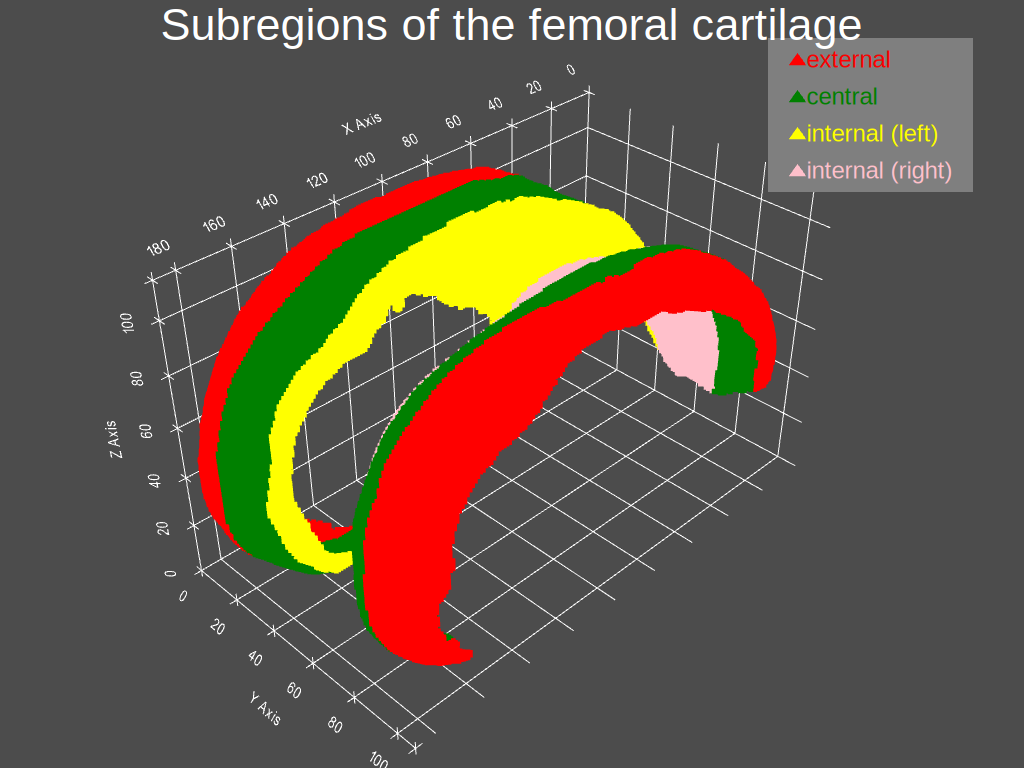
\includegraphics[width=\linewidth]{./figures/femoral_subregions}
	\caption{Subregions of the femoral cartilage. Color codes are as follows: red - lateral anterior; green - medial anterior; orange - lateral central; cyan - medial central; purple - lateral posterior; yellow - medial posterior}
	\label{fig:femoral_subregions}
\end{figure}
\begin{figure}[]
	\centering
	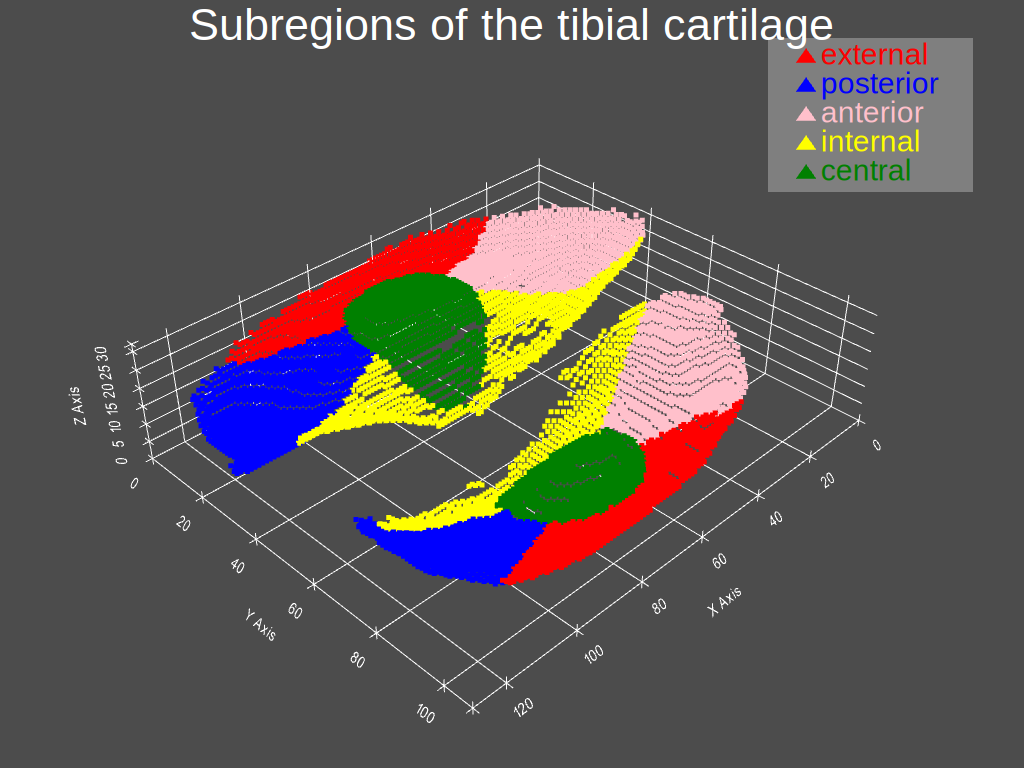
\includegraphics[width=\linewidth]{./figures/tibial_subregions}
	\caption{Subregions of the tibial cartilage. Color codes are as follows: red - internal; green - anterior; orange - posterior; blue - external; pink - central}
	\label{fig:tibial_subregions}
\end{figure}
	\section{Splitting of femoral cartilage}
\label{sec:Splitting}
As mentioned earlier, the femoral cartilage is split into multiple parts, namely the central weight-bearing zones, the anterior and the posterior sections (of the lateral and medial cartilage, respectively). The weight-bearing zones are defined as those regions of the cartilage which lie vis-a-vis, i.e. are in contact with, the central regions of the tibial cartilage (cLT/cMT, eLT/eMT, iLT/iMT). Once these are extracted, definition of the anterior and posterior parts is trivial: they are what is left of the cartilage on either side of the central weight-bearing zones (Refer to figure \ref{fig:femoral_subregions}). To circumvent the problem the convex nature of the posterior parts poses to mesh triangulation and function fitting, these sections are rotated by 90°. 
\par\noindent
Let the lateral and medial tibial cartilage plates be represented by two point clouds $LT$ and $MT$. Furthermore, let the central, external and internal subregions of the plates be represented by points clouds $cLT$, $eLT$, $iLT \subset LT$ and $cMT$, $eMT$, $iMT \subset MT$. For both point clouds, subsets $LT' \subset LT$ and $MT' \subset MT$ are defined such that
\newline
\begin{equation}
	LT' := \{\:(x,y,z)_i \in LT \:|\: x < \max_{x} cLT \land x > \min_{x} cLT\:\}
\end{equation}
\begin{equation}
	MT' := \{\:(x,y,z)_i \in MT \:|\: x < \max_{x} cMT \land x > \min_{x} cMT\:\}
\end{equation}
\newline
These subsets represent the parts of the tibial cartilage plates in contact with the femoral cartilage (in standing position). They can then be used to extract the corresponding parts of the femoral cartilage. Let the lateral and medial femoral cartilage regions be represented by two points clouds $LF$ and $MF$. For both point clouds, subsets $LF' \subset LF$ and $MF' \subset MF$ are defined such that
\newline
\begin{equation}
	LF' := \{\:(x,y,z)_i \in LF \:|\: x < \max_{x} LT' \land x > \min_{x} LT' \land y < \max_{y} LT' \land y > \min_{y} LT'\:\}
\end{equation}
\begin{equation}
	MF' := \{\:(x,y,z)_i \in MF \:|\: x < \max_{x} MT' \land x > \min_{x} MT' \land y < \max_{y} MT' \land y > \min_{y} MT'\:\}
\end{equation}
\newline
These subsets represent the parts of the femoral cartilage in contact with the tibial cartilage (in standing position), i.e. the central weight-bearing zones of the femoral cartilage.
\par\noindent
As mentioned before, definition of the remaining subregions of the femur is then trivial. Let the lateral and medial anterior and posterior regions of the femoral cartilage be represented by point clouds $aLF$, $pLF \subset LF$ and $aMF$, $pMF \subset MF$ such that
\newline
\begin{equation}
	aLF := \{\:(x,y,z)_i \in LF \:|\: x < \min_{x} LF'\:\}
\end{equation}
\begin{equation}
	aMF := \{\:(x,y,z)_i \in MF \:|\: x < \min_{x} MF'\:\}
\end{equation}
\begin{equation}
	pLF := LF \setminus (LF' \cup aLF)
\end{equation}
\begin{equation}
	pMF := MF \setminus (MF' \cup aMF)
\end{equation}
\newline
The subregions of the central weight-bearing zones are determined as suggested by \cite{wirth2008technique}.
	\section{Acronyms}
	\begin{acronym}
		\acro{ecLF}{Mean thickness of the external cartilage subregion of the central part of the lateral femoral condyle}
		\acro{ccLF}{Mean thickness of the central cartilage subregion of the central part of the lateral femoral condyle}
		\acro{icLF}{Mean thickness of the internal cartilage subregion of the central part of the lateral femoral condyle}
		\acro{icMF}{Mean thickness of the internal cartilage subregion of the central part of the medial femoral condyle}
		\acro{ccMF}{Mean thickness of the central cartilage subregion of the central part of the medial femoral condyle}
		\acro{ecMF}{Mean thickness of the external cartilage subregion of the central part of the medial femoral condyle}
		\acro{cLT}{Mean thickness of the central cartilage subregion of the lateral tibia}
		\acro{aLT}{Mean thickness of the anterior cartilage subregion of the lateral tibia}
		\acro{eLT}{Mean thickness of the external cartilage subregion of the lateral tibia}
		\acro{pLT}{Mean thickness of the posterior cartilage subregion of the lateral tibia}
		\acro{iLT}{Mean thickness of the internal cartilage subregion of the lateral tibia}
		\acro{cMT}{Mean thickness of the central cartilage subregion of the medial tibia}
		\acro{aMT}{Mean thickness of the anterior cartilage subregion of the medial tibia}
		\acro{eMT}{Mean thickness of the external cartilage subregion of the medial tibia}
		\acro{pMT}{Mean thickness of the posterior cartilage subregion of the medial tibia}
		\acro{iMT}{Mean thickness of the internal cartilage subregion of the medial tibia}
		\acro{x.aSD}{Standard deviation of the thickness of the respective (x) cartilage subregion}
		\acro{x.aMav}{Mean value of the maximum 1\% measurements of cartilage thickness of the respective (x) cartilage subregion}
		\acro{x.aMiv}{Mean value of the minimum 1\% measurements of cartilage thickness of the respective (x) cartilage subregion}
	\end{acronym}
	
	\bibliographystyle{alpha}
	\bibliography{sources}
	
\end{document}

